% !TeX program = xelatex
% Overleaf: Menu → Compiler → XeLaTeX；主文件设为 latex/main.tex
\documentclass[UTF8,a4paper,11pt,fontset=fandol]{ctexart}
% Overleaf: Compiler = XeLaTeX
\usepackage{graphicx}
\usepackage{booktabs}
\usepackage{enumitem}
\usepackage{xcolor}
\usepackage{amsmath}
\usepackage{amssymb}
\usepackage{tabularx}
\usepackage{fancyhdr}
\usepackage{titlesec}
\usepackage{xurl}
\usepackage{hyperref}

\hypersetup{
  colorlinks=true,
  linkcolor=blue!60!black,
  urlcolor=blue!70!black,
  citecolor=blue!60!black,
  breaklinks=true
}

\pagestyle{fancy}
\fancyhf{}
\fancyhead[L]{\small 课题组科研入门手册}
\fancyhead[R]{\small\nouppercase{\leftmark}}
\fancyfoot[C]{\thepage}
\renewcommand{\headrulewidth}{0.4pt}
\renewcommand{\footrulewidth}{0pt}

\setlist[itemize]{leftmargin=*,itemsep=2pt,topsep=4pt}
\setlist[enumerate]{leftmargin=*,itemsep=2pt,topsep=4pt}

\newcommand{\resurl}[1]{\url{#1}}
\newcommand{\tipbox}[1]{%
  \par\vspace{4pt}\noindent\textbf{要点：}#1\par\vspace{4pt}%
}


\title{\textbf{课题组科研入门手册}\\[0.6em]
\large 深度学习 · 计算机视觉 · 医学影像 AI}
\author{组内学习资料整理版}
\date{\today}

\begin{document}
\maketitle
\begin{abstract}
\noindent
本手册面向新加入课题组的本科生与研究生，整合组内既有学习笔记、学长经验分享、学术交流纪要与工具链接，形成可在 Overleaf 协作编辑、并在 GitHub 按路径自学的入门材料。阅读建议：先看第~1~章与仓库 \texttt{README} 中的周计划，再按章节推进；链接与模板以仓库最新版本为准。
\end{abstract}

\tableofcontents
\newpage

\section{导读与能力目标}

\subsection{手册怎么用}
本手册与 GitHub 仓库配套使用：
\begin{itemize}
  \item \textbf{自学入口}：仓库根目录 \texttt{README.md}（周计划、Overleaf 同步说明）。
  \item \textbf{正文}：本 LaTeX 手册（\texttt{latex/}），可在 Overleaf 在线改、编译 PDF。
  \item \textbf{模板与清单}：\texttt{templates/}、\texttt{assets/reading-list/}。
\end{itemize}

\subsection{入门后应具备的能力}
完成 4--8 周入门路径后，期望你能够：
\begin{enumerate}
  \item 用关键词在 Google Scholar / 顶会官网检索文献，并维护一份结构化文献 list；
  \item 按「泛读→筛选→精读→笔记」读完领域综述与 1--2 篇经典论文；
  \item 用 PyTorch 跑通官方入门示例，并读懂一份规范开源仓库的目录结构；
  \item 独立完成一次组会汇报（论文汇报或周汇报），并保留实验/会议记录；
  \item 说清自己课题的问题定义、输入输出、评价指标与数据来源（哪怕仍很初步）。
\end{enumerate}

\subsection{建议的时间节奏（概览）}
\begin{center}
\begin{tabular}{clp{8cm}}
\toprule
阶段 & 时长 & 重点 \\
\midrule
环境与框架 & 第 1 周 & PyTorch 60 分钟教程、开发环境、Claude Code 入门 \\
文献方法 & 第 2--3 周 & 检索渠道、综述精读、文献 list、Zotero \\
经典模型 & 第 4--5 周 & ResNet / Transformer 等精读 + 代码浏览 \\
课题对齐 & 第 6--7 周 & 组内课题范式、数据集摸底、第一次正式汇报 \\
巩固输出 & 第 8 周 & 复现小实验、整理笔记、制定下阶段 roadmap \\
\bottomrule
\end{tabular}
\end{center}

更细的逐周 checklist 见仓库 \texttt{README.md}；可复制 \path{templates/learning_plan.md} 填写个人计划。

\subsection{三个一定（贯穿全程）}
\begin{enumerate}
  \item \textbf{论文读完一定要做笔记}：方法归纳、贡献、未解决问题、对自己课题的启发。
  \item \textbf{实验跑完一定要有记录}：时间、软硬件、代码版本、数据、结果、分析、下一步。
  \item \textbf{组会一定要有纪要 + 待办}：把老师和同学指出的问题落到下一阶段任务。
\end{enumerate}

\section{科研心态与基本规范}

\subsection{科研与上课的差别}
做科研通常没有现成教科书可逐步照做，主要依靠文献检索、批判性阅读、实验验证与反复修改。进展慢、卡住、被拒稿都很常见；关键是建立可持续的习惯，而不是追求短期「看起来很忙」。

\subsection{能力与态度}
结合组内学长与学术交流共识，入门阶段尤其需要：
\begin{itemize}
  \item \textbf{主动性}：主动查文献、主动问清任务边界、事事有回音；
  \item \textbf{自主学习}：会用检索与社区资源，并能归纳总结；
  \item \textbf{抗挫折}：论文读不懂、代码跑不通、实验不涨点是常态；
  \item \textbf{时间管理}：期刊周期常要数月，需提前为写作与返修留时间；
  \item \textbf{身心健康}：科研只是生活的一部分；适当运动有助于长期效率。
\end{itemize}

\subsection{常见误区}
\begin{enumerate}
  \item \textbf{「顶会/顶刊文章一定都对」}：带批判性阅读；A 类未必处处优于 B 类，没有工作是完美的。
  \item \textbf{「调参总能调出好结果」}：好模型不应只靠黑箱撞运气；单组参数极好而其他组都崩，往往意味着错误或偶然性，需警惕。
  \item \textbf{「模型越复杂越好」}：优先抓住核心创新与可解释动机，避免为复杂而复杂。
  \item \textbf{「不清楚自己解决了什么问题」}：投稿前反复自问：真问题是什么？技术贡献是什么？读者能带走什么？切忌编造问题。
\end{enumerate}

\subsection{选题与问题价值（交流纪要精华）}
确定方向前，建议先想清楚：
\begin{itemize}
  \item 问题为什么重要？现有方法为什么解决不好？
  \item 自己为什么有机会解决（数据、算力、团队积累）？
  \item 能否逐步形成一条研究主线，而不是互不相关的零散文章？
\end{itemize}
有价值的问题往往来自长期看数据、做实验、接触真实场景，而不是简单从别人 limitation 里「抄一个缺口」。换方法、换技术点可以，但尽量避免频繁更换大方向。

\subsection{何时收尾、如何面对拒稿}
\begin{itemize}
  \item 论文没有绝对完美版。若问题讲清、方法合理、关键实验稳定、结论可支撑，就应整理投稿，而不是无限打磨。
  \item 拒稿是常态。有道理的意见认真改；不合理的意见不必过度内耗。rebuttal 要判断工作本身是否够强、负面意见是否可正面回应。
\end{itemize}

\subsection{硕士阶段可落地的启发}
\begin{enumerate}
  \item 困难是常态，不要因短期无成果否定自己。
  \item 选题兼顾兴趣、问题价值、资源与可行性。
  \item 写作重在把问题—方法—实验—贡献讲清楚。
  \item 尽早形成文献阅读、实验记录、阶段总结、定期汇报的习惯。
  \item 从真实问题出发，而不是为了发文而堆方法。
\end{enumerate}

\section{文献检索、阅读与汇报}

\subsection{检索渠道}
\begin{itemize}
  \item 中文入门：知网优质综述（适应英文前可先建立领域地图）。
  \item 英文主渠道：Google Scholar、\texttt{arxiv.org}、AMiner（\url{https://www.aminer.cn/}）、PubScholar（\url{https://pubscholar.cn/}）。
  \item 代码与论文绑定：Papers with Code（\url{https://paperswithcode.com/}）。
  \item 引用关系可视化：Connected Papers、Open Knowledge Maps（\url{https://openknowledgemaps.org/}）。
  \item 会议/期刊权威性：参考 CCF 列表；组内常用投稿目标见图~\ref{fig:journal-list}。
\end{itemize}

\begin{figure}[htbp]
  \centering
  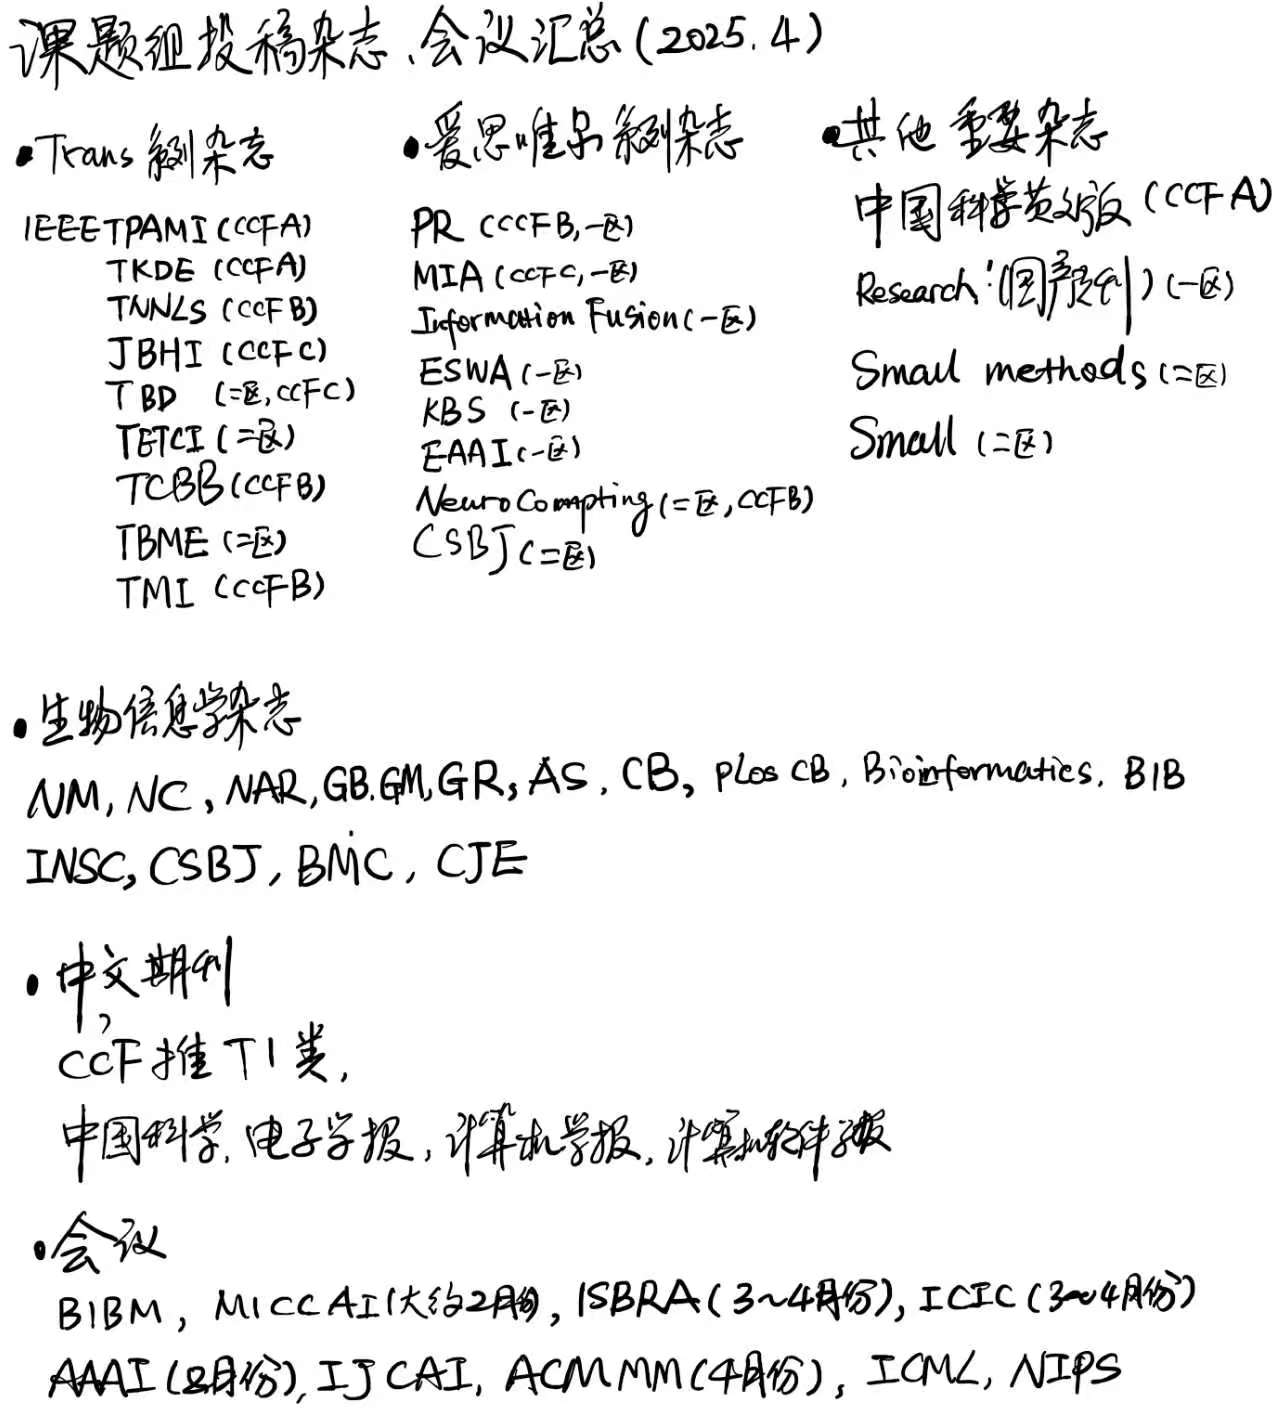
\includegraphics[width=0.92\textwidth]{figures/journal_list.jpg}
  \caption{课题组投稿期刊/会议汇总示意（以组内最新版本为准）}
  \label{fig:journal-list}
\end{figure}

\subsection{优先关注的顶刊顶会入口}
调研相关工作时，优先从以下来源筛选（完整链接见第~8~章）：
PR、IEEE TPAMI、TIP、IEEE TNNLS、AAAI、CVPR、ECCV、ICCV、ACM MM、NeurIPS 等。
常用开放获取入口示例：
\begin{itemize}
  \item CVPR 2024：\url{https://openaccess.thecvf.com/CVPR2024}
  \item ECCV：\url{https://www.ecva.net/papers.php}
  \item ICCV：\url{https://openaccess.thecvf.com/ICCV2023}
  \item TIP / TPAMI：IEEE Xplore 期刊近期论文页
\end{itemize}

\subsection{文献筛选策略}
\begin{enumerate}
  \item 先读\textbf{英文综述}：主流方法、开放问题、数据集、指标、前景。
  \item 再筛论文：经典 / 顶会顶刊 / 有代码有数据者优先；无代码也可借鉴思想与 trick。
  \item 看不懂时：知乎、B 站、油管上的论文/代码解读可作辅助，但结论需回原文核对。
\end{enumerate}

\subsection{建立文献 List（强制习惯）}
每条记录建议至少包含：题目、作者、引用量、发表时间、链接、有无代码及链接、有无数据集及链接。
可复制仓库模板：\path{templates/literature_list.csv}；范例清单见 \path{assets/reading-list/}。

\subsection{阅读顺序与精读目标}
\textbf{泛读顺序：} Abstract + 文中第一张总览图 $\rightarrow$ Introduction $\rightarrow$ Conclusion；\\
确有继续价值再读 Method $\rightarrow$ Experiment。

精读一篇后，应能讲清：
\begin{itemize}
  \item 问题定义（输入/输出、指标、数据）；
  \item 背景与现有方法不足；
  \item 研究动机与方法框架；
  \item 主要实验结论与 contribution；
  \item 对你课题的可迁移点。
\end{itemize}
\tipbox{读第一篇领域论文不要过于乐观，真正读懂常需 1--2 周；读懂一篇往往要连带读十余篇相关工作，这是正常现象。}

文献管理推荐：Zotero（可配合坚果云同步）。笔记可用 Obsidian / Notion。

\subsection{论文汇报 Checklist}
汇报一篇论文时，建议覆盖：
\begin{enumerate}
  \item Background：为什么有必要做；
  \item Challenge：技术/应用难点；
  \item Existing methods：已有路线与不足；
  \item Method：核心思路与框架图；
  \item Dataset \& metrics；
  \item Results：对比与消融；
  \item Conclusion + 你的批判性思考与下一步。
\end{enumerate}
扫描版要点图册见仓库 \texttt{assets/tips/literature\_and\_report\_tips.pdf}。

\subsection{周汇报 Checklist}
\begin{itemize}
  \item 上周遗留问题是否解决；
  \item 本周具体工作（文献/代码/实验/写作）；
  \item 本周卡点与已尝试的排查；
  \item 下周计划与需要的支持。
\end{itemize}
模板：\texttt{templates/weekly\_report.md}。

\section{代码能力与 AI 辅助开发}

\subsection{深度学习框架入门（PyTorch）}
必须掌握至少一种主流框架；本组默认推荐 PyTorch。
\begin{itemize}
  \item 官方 60 分钟速成：\url{https://pytorch.org/tutorials/beginner/deep_learning_60min_blitz.html}
  \item 中文解读参考：\url{https://zhuanlan.zhihu.com/p/86875507}
  \item 大模型相关 PyTorch 入门（视频号 CS336 相关分享）：可在微信视频号检索「斯坦福 CS336 PyTorch」
\end{itemize}
配套练习：李沐《动手学深度学习》B 站课程：\\
\url{https://www.bilibili.com/video/BV1if4y147hS/}

建议路径：官方 tutorial $\rightarrow$ 复现一个小模型（如 MNIST/CIFAR）$\rightarrow$ 阅读领域经典开源实现。

\subsection{推荐的工程目录布局}
阅读或自建训练仓库时，可参考如下结构：
\begin{itemize}
  \item \texttt{config/}：训练超参、路径配置；
  \item \texttt{dataset/} 或 \texttt{dataloader/}：数据读取与增强；
  \item \texttt{models/}：网络模块；
  \item \texttt{metrics/}：损失与评价指标；
  \item \texttt{utils/}：通用工具；
  \item \texttt{scripts/}：训练/评测启动脚本（服务器可用 \texttt{nohup}，集群可用 \texttt{sbatch}）；
  \item \texttt{weights/}： checkpoint；
  \item \texttt{train.py}：主入口。
\end{itemize}

\subsection{如何找论文对应代码}
\begin{enumerate}
  \item 论文摘要/介绍末尾的 GitHub 链接；
  \item 用项目名在 GitHub 搜索；
  \item Papers with Code 按论文名检索；
  \item 必要时礼貌邮件作者（说明身份与用途）。
\end{enumerate}
工业界代码更新快、社区强，但医学场景未必开箱即用；医学专用代码更贴数据，但维护与数据公开性可能较弱。建议各选一份高质量实现精读模仿。

\subsection{读代码的检查清单}
\begin{itemize}
  \item 任务定义：源码要解决什么问题；
  \item 数据：类型、路径、预处理；
  \item 环境：依赖、版本、硬件；
  \item 能否跑通、输出是什么；
  \item 整体架构与关键模块对应论文哪一段。
\end{itemize}

\subsection{Claude Code / AI 辅助编程}
AI 适合辅助写样板代码、解释报错、阅读陌生仓库；但\textbf{不能}替代你对方法与实验的理解，生成内容必须核对。
入门资料：
\begin{itemize}
  \item 完全指南：\url{https://mp.weixin.qq.com/s/5uhudUPNKLYwxZXB0_IH_g}
  \item 命令与工作流：\url{https://mp.weixin.qq.com/s/pwozo7PSu8RGedfzs0E6BA?scene=1}
  \item 背景阅读：\url{https://mp.weixin.qq.com/s/YHDSJayeDwmtqY1pGT9MnA}
\end{itemize}
练习建议：先学会清晰下指令（目标、约束、文件范围），再让 AI 解释/改错，最后自己跑通并写进实验记录。

\subsection{训练与调试习惯}
\begin{itemize}
  \item 每次尽量只改一个变量，便于归因；
  \item 监控损失与关键指标，区分过拟合/欠拟合；
  \item 保存随机种子、配置文件与代码 commit，保证可复现；
  \item 困难时按「数据质量 $\rightarrow$ 预处理 $\rightarrow$ 增强 $\rightarrow$ 结构 $\rightarrow$ 超参 $\rightarrow$ 预训练/迁移」排查。
\end{itemize}

\section{Idea、实验与时间规划}

\subsection{一条常见的阶段时间表}
\begin{center}
\begin{tabular}{clp{7.2cm}}
\toprule
阶段 & 约需时间 & 任务 \\
\midrule
想 idea & 1--2 个月 & 规划任务、发现 technical challenge / failure case、构思解法 \\
做实验 & 2--3 个月 & 简单实验验证 $\rightarrow$ 简单数据改进 $\rightarrow$ 真实数据调通 \\
写论文 & 约 1 个月 & 按投稿节点倒排、写作、自查、修改 \\
\bottomrule
\end{tabular}
\end{center}
实际往往更长；假期与课余集中时间对前期积累尤其重要。

\subsection{两种科研推进方式}
\paragraph{Idea-driven（跟进式）}
看到有趣的 SOTA，发现 failure case，提出新算法修补。\\
优点：上手快，适合新手。\\
缺点：影响力依赖提升幅度；易撞车；创新空间受原任务束缚。

\paragraph{Goal-driven（目标牵引）}
先设定长期目标与 roadmap，再选任务、挖 failure case、设计解法。\\
优点：更易做出成体系、有动机的工作。\\
缺点：规划 roadmap 本身很难，需要导师指导与领域积累。

\subsection{如何发现与解决 Failure Cases}
\begin{enumerate}
  \item 探索算法上限，在更难 case / 新数据设定上找失败模式；
  \item 把表面现象抽象成真正的 technical challenge；
  \item 从自己的「武器库」（可复用的 technique / insight）中组合解法；
  \item 好的工作往往不是简单 A+B，而是把 A 与 B 巧妙结合。
\end{enumerate}
当领域出现「新锤子」（如扩散模型、大模型范式）时，用它去推进自己 roadmap 上的里程碑，常更容易做出有影响力的工作。

\subsection{实验策略：先简单后真实}
\textbf{简单实验}：尽量只保留你要验证的那个 core challenge，排除无关干扰，先证明解法「在该挑战上 work」。\\
然后再到真实数据上把系统调通，并补齐对比与消融。

\subsection{实验记录最低要求}
日期、步骤、想法、失败实验、配置、结果图表、下一步计划，都应可回溯。实验记录是成果的原始证据。

\subsection{经典模型精读清单（代码与论文）}
建议结合李沐论文精读仓库：\url{https://github.com/mli/paper-reading}\\
优先顺序示例：ResNet $\rightarrow$ Transformer $\rightarrow$ GAN $\rightarrow$ 对比学习 $\rightarrow$ Swin Transformer $\rightarrow$ CLIP $\rightarrow$ Two-Stream $\rightarrow$ 多模态学习。

\section{论文写作与科研工具箱}

\subsection{写作心态}
论文写作更像「有逻辑的论证」：证明工作有意义、方法合理、证据充分。句式往往相对固定，难点在逻辑链条与贡献叙事。恪守学术诚信；多听写作讲座、多模仿优秀论文结构。

\subsection{写作与协作平台}
\begin{itemize}
  \item Overleaf：组内默认 LaTeX 协作平台（本手册即可在 Overleaf 编辑）。
  \item 表格：TableGenerator 等在线工具。
  \item 润色：DeepL（翻译）、Grammarly（语法，注意学术表述仍需人工把关）。
\end{itemize}

\subsection{画图}
\begin{itemize}
  \item 流程图：draw.io（免费易上手）、Visio、diagrams；
  \item 精修矢量：Adobe Illustrator；
  \item PPT 作图后导出 PDF 插入 LaTeX，文字可清晰；
  \item AI 辅助科研示意图 MCP（需自行评估适用性）：\\
        \url{https://github.com/icebird1998/drawio-scientific-illustrator}
\end{itemize}
TIP 等期刊对图表风格有规范要求，组内相关材料请向导师/师兄索取最新版；写稿时统一字体、线宽、配色与编号。

\subsection{文献与实验周边工具}
\begin{itemize}
  \item 文献管理：Zotero；
  \item 训练可视化：Weights \& Biases；模型与数据集社区：Hugging Face；
  \item 笔记与日程：Notion / Obsidian；
  \item 预印本：arXiv（增加曝光，但需批判性阅读未经审稿内容）；
  \item 匿名开源：Anonymous GitHub（\url{https://anonymous.4open.science/}）。
\end{itemize}

\subsection{AI 读论文助手}
Paper Copilot（\url{https://papercopilot.com/}）等可用于快速扫文、提炼对比表；\textbf{结论与引用必须人工核对}，不可直接当作事实写入论文。

\subsection{投稿截止时间}
\begin{itemize}
  \item CCF 会议倒计时：\url{https://ccfddl.top/}
  \item AI deadlines：\url{https://github.com/abhshkdz/ai-deadlines} 及社区维护镜像
\end{itemize}
务必区分摘要截止与全文截止，并注意时区。

\subsection{优秀开源仓库的特征}
清晰说明、可视化结果、便于复现、排版有序；论文与 GitHub 互相引用（盲审阶段除外）。

\section{组内课题范式：医学影像 AI 问题拆解}

本章抽象自组内「医学影像辅助检测」类课题梳理经验，重点示范\textbf{如何把模糊课题拆成可研究、可验证的子问题}，不绑定具体项目名称或未公开数据。

\subsection{从临床诉求到系统定位}
典型临床痛点包括：阅片疲劳导致漏诊、微小/隐匿病灶难发现、报告标准不统一。\\
对应系统目标常包括：提高检出、缩短报告时间、统一标准、控制假阳性。\\
入门时先分清能力层级，例如：
\begin{enumerate}
  \item \textbf{提质增效}：阅片前自动检测与标记（CADe）——多数入门课题先落在此层；
  \item \textbf{智能预警}：高风险病灶优先级提醒；
  \item \textbf{高级辅助}：诊断建议、结构化报告、复杂决策支持。
\end{enumerate}
写开题/汇报时明确边界：辅助检出 $\neq$ 替代诊断。

\subsection{技术本质常见画像}
医学影像检测问题常同时具备：
\begin{itemize}
  \item \textbf{小目标}：病灶尺度小、信号弱；
  \item \textbf{异常检测}：低对比、位置隐匿；
  \item \textbf{极度类别不平衡}：正常体素远多于病灶。
\end{itemize}
不同病种在模态（CT/MRI/X-ray）、维度（2D/3D）与外观上差异大，可能需要多任务学习或病种专用检测器——选题时先做数据与任务摸底。

\subsection{推荐的子问题拆解框架}
可将 pipeline 正交拆成若干可独立调研的子问题，例如：
\begin{enumerate}
  \item \textbf{弱信号保留}：下采样中如何保住微小病灶特征？多尺度如何融合？
  \item \textbf{召回--假阳性权衡}：高召回下如何把 FPR 压到临床可接受区间？
  \item \textbf{多模态语义}：病史/报告文本与影像如何对齐？结构化输出如何保证事实准确？
  \item \textbf{工程部署}：精度与时延/边缘算力如何权衡？如何接入现有工作流？
  \item \textbf{数据与标注}：标注稀缺、不一致、不平衡如何缓解（弱监督/半监督等）？
  \item \textbf{评价体系}：如何定义并衡量「诊断质量提升」，而不只是刷单一指标？
\end{enumerate}
\tipbox{先把「问题」与「具体网络结构方案」分开写。级联网络、某损失等是手段，不应在问题尚未清晰时就锁死方案。}

\subsection{入门四周可执行的下一步}
\begin{enumerate}
  \item 针对你被分配的 1--2 个子问题，各检索若干 SOTA 与开源基准；
  \item 数据摸底：公开/可申请数据、标注规模与许可；
  \item 与导师确认首个切入点与成功标准（指标与临床约束）；
  \item 用第~3~章模板产出文献 list，并做一次 15--20 分钟汇报。
\end{enumerate}

\subsection{数据集检索入口}
\begin{itemize}
  \item Nature Scientific Data：\url{https://www.nature.com/sdata/}
  \item Grand Challenge（医学影像竞赛数据）：\url{https://grand-challenge.org/}
  \item Kaggle Datasets：\url{https://www.kaggle.com/datasets}
  \item Papers with Code 数据集页；以及从顶会论文中挖作者公开数据。
\end{itemize}
使用前务必阅读许可协议、获取门槛与标注说明。数据集整理字段模板见 \texttt{templates/dataset\_sheet.csv}。

\section{资源总表}

\subsection{PyTorch 与基础课}
\begin{itemize}
  \item \url{https://pytorch.org/tutorials/beginner/deep_learning_60min_blitz.html}
  \item \url{https://zhuanlan.zhihu.com/p/86875507}
  \item 动手学深度学习（B 站）：\url{https://www.bilibili.com/video/BV1if4y147hS/}
  \item 李沐论文精读：\url{https://github.com/mli/paper-reading}
\end{itemize}

\subsection{组内科研经验分享（录像/网盘）}
\begin{itemize}
  \item 科研简略 I（百度网盘）：\url{https://pan.baidu.com/s/1tK9uESAtxD_yijJwGErGqA?pwd=wb3n}（提取码 wb3n）
  \item 科研简略 II（腾讯会议录制）：\url{https://meeting.tencent.com/v2/cloud-record/share?id=22ddba59-56f0-4401-9ab0-ae56d99689b0&from=3}（密码 KYJL）
  \item 本科生/研究生科研技能分享：\url{https://meeting.tencent.com/v2/cloud-record/share?id=b44b2452-2c32-4479-88be-895946030b87&from=3&is-single=false&record_type=2}（密码 2024）
\end{itemize}
若链接失效，请向课题组管理员索取最新地址。

\subsection{顶会顶刊与论文列表}
\begin{itemize}
  \item 个人/社区汇总页示例：\url{https://github.com/jiandanjinxin/jiandanjinxin.github.io}
  \item CVPR 2024：\url{https://openaccess.thecvf.com/CVPR2024}
  \item CVPR 论文汇总仓库：\url{https://github.com/DmitryRyumin/CVPR-2023-24-Papers}
  \item ECCV 论文列表（Paper Copilot）：\url{https://papercopilot.com/paper-list/eccv-paper-list/eccv-2024-paper-list/}
  \item ECCV 官方：\url{https://www.ecva.net/papers.php}
  \item ICCV 开放获取：\url{https://openaccess.thecvf.com/ICCV2023}
  \item ICCV 汇总仓库：\url{https://github.com/DmitryRyumin/ICCV-2023-Papers}
  \item IEEE TIP：\url{https://ieeexplore.ieee.org/xpl/RecentIssue.jsp?punumber=83}
  \item IEEE TPAMI：\url{https://ieeexplore.ieee.org/xpl/RecentIssue.jsp?punumber=34}
\end{itemize}

\subsection{数据集与竞赛}
\begin{itemize}
  \item \url{https://www.nature.com/sdata/}
  \item \url{https://grand-challenge.org/}
  \item \url{https://www.kaggle.com/} \quad \url{https://www.kaggle.com/datasets}
  \item \url{https://paperswithcode.com/}
\end{itemize}

\subsection{AI 辅助与绘图}
\begin{itemize}
  \item Claude Code 指南：\url{https://mp.weixin.qq.com/s/5uhudUPNKLYwxZXB0_IH_g}
  \item Claude Code 工作流：\url{https://mp.weixin.qq.com/s/pwozo7PSu8RGedfzs0E6BA?scene=1}
  \item Paper Copilot：\url{https://papercopilot.com/}
  \item 科研绘图 MCP：\url{https://github.com/icebird1998/drawio-scientific-illustrator}
  \item CCF DDL：\url{https://ccfddl.top/}
\end{itemize}

\subsection{微信公众号（可选订阅）}
\begin{itemize}
  \item 多模态机器学习与大模型（\texttt{multimodal-ml1218}）
  \item 多模态论文每日速递（\texttt{MultimodlPaper}）
  \item Ai 医影多模态组学（\texttt{aimedicalimage}）
\end{itemize}

\subsection{延伸阅读建议}
\begin{itemize}
  \item 多模态学习综述类推文示例：\url{https://mp.weixin.qq.com/s/_Q1BBPYF0_xnVzqmVXdkJQ}（阅读后仍应回到原始论文核对）
  \item 仓库内阅读清单范例：\texttt{assets/reading-list/}
\end{itemize}

\vspace{1em}
\noindent\textit{手册内容来源于组内既有笔记与公开链接的系统化整理，随仓库迭代更新。欢迎提交 Issue / Pull Request 修正失效链接或补充经验。}


\end{document}
